\documentclass[a4paper,12pt]{article}

% --- Базовые пакеты ---
\usepackage[russian]{babel}
\usepackage[T2A]{fontenc}
\usepackage[utf8]{inputenc}
\usepackage{geometry}
\usepackage{amsmath, amssymb}
\usepackage{graphicx}
\usepackage{cancel}
\usepackage{float} 
\usepackage{xcolor}
\usepackage{array}
\usepackage{caption}
\usepackage{booktabs}
\usepackage{subcaption}
\usepackage{pgfplots}
\pgfplotsset{compat=1.18}
\usetikzlibrary{arrows.meta, matrix, positioning}
\usepackage{capt-of}
\usepackage{multirow}
\usepackage[siunitx]{circuitikz}
\usepackage[bottom]{footmisc}
\usepackage{tcolorbox}
\usepackage{nicematrix}
\usepackage{tikz}

% --- Гиперссылки (ОДИН РАЗ!) ---
\usepackage{hyperref}
\hypersetup{
	colorlinks=true,
	linkcolor=red,
	citecolor=red,
	urlcolor=red,
	filecolor=red,
	linktoc=page
}

% --- Содержание ---
\usepackage{tocloft}
\usepackage{etoolbox}

% Патчим \tableofcontents для черного текста и красных номеров страниц
\preto\tableofcontents{%
	\begingroup
	\renewcommand{\contentsline}[4]{%
		\ifnum\pdfstrcmp{##1}{section}=0
		\vskip 4pt{\normalfont\color{black}##2}\nobreak\hfill
		{\normalfont\color{red}\hyperlink{##4}{##3}}\par
		\else\ifnum\pdfstrcmp{##1}{subsection}=0
		\vskip 2pt\hspace{1.5em}{\normalfont\color{black}##2}\nobreak\hfill
		{\normalfont\color{red}\hyperlink{##4}{##3}}\par
		\else
		\vskip 1pt\hspace{3em}{\normalfont\color{black}##2}\nobreak\hfill
		{\normalfont\color{red}\hyperlink{##4}{##3}}\par
		\fi\fi
	}%
}
\appto\tableofcontents{\endgroup}

% --- Листинги MATLAB ---
\usepackage{listings}
\usepackage{matlab-prettifier} % <-- Подключаем пакет

% Цвета
\definecolor{codebg}{RGB}{250,250,252}
\definecolor{linenumcolor}{RGB}{150,150,170}
\definecolor{matlabblue}{RGB}{0,0,200}
\definecolor{matlabgreen}{RGB}{30,130,30}
\definecolor{matlaborange}{RGB}{200,80,0}

% Настройка matlab-prettifier (НЕ через \lstset{style=...})
\lstset{
	style              = Matlab-editor, % Стиль пакета
	basicstyle         = \mlttfamily\small, % ВАЖНО: шрифт из пакета
	backgroundcolor    = \color{codebg},
	frame              = single,
	frameround         = tttt,
	framesep           = 4pt,
	rulecolor          = \color{matlabblue!30},
	numbers            = left,
	numberstyle        = \tiny\color{linenumcolor},
	numbersep          = 10pt,
	breaklines         = true,
	tabsize            = 4,
	showstringspaces   = false,
	captionpos         = b,
	xleftmargin        = 15pt,
	xrightmargin       = 5pt,
	escapeinside       = {\%*}{*)},
}

% Настройки подписей листингов
\renewcommand{\lstlistingname}{Листинг}
\DeclareCaptionFormat{redlisting}{#1\textcolor{red}{#2}#3}
\captionsetup[lstlisting]{format=redlisting}

% --- Геометрия и общие настройки ---
\geometry{left=1.5cm, right=2cm, bottom=2cm, top=2cm}
\captionsetup[figure]{name=Рисунок}
\captionsetup[table]{name=Таблица}
\captionsetup{labelsep=endash}
\newcommand{\figwidth}{0.5\textwidth}


\begin{document}

\begin{titlepage}
\centering

\vspace*{0.5cm}
{\small
Министерство науки и высшего образования Российской Федерации\\[2pt]
Федеральное государственное автономное образовательное учреждение\\
высшего образования\\[2pt]
\textbf{«Национальный исследовательский университет ИТМО»}\\
}

\vspace{0.8cm}
\hrule height 0.8pt
\vspace{0.3cm}

{\large Факультет систем управления и робототехники}

\vspace{0.3cm}
\hrule height 0.4pt
\vspace{2.5cm}

{\Huge\bfseries ОТЧЁТ}\\[0.4cm]
{\LARGE\bfseries о лабораторной работе №1}\\[0.8cm]

\begin{tcolorbox}[
colback=gray!4,
colframe=gray!10,
boxrule=0.8pt,
arc=4pt,
left=12pt, right=12pt, top=8pt, bottom=8pt
]
\centering
{\large По дисциплине:\\[4pt]}
{\large\bfseries «Нелинейные системы управления»}\\[10pt]
\end{tcolorbox}

\vspace{5cm}

\begin{minipage}{0.45\textwidth}
\raggedright
{\large\bfseries Студенты:}\\[4pt]
Охрименко Е.\,Д.\\
Титаренко П. А.
\end{minipage}
\hfill
\begin{minipage}{0.45\textwidth}
\raggedleft
{\large\bfseries Преподаватель:}\\[4pt]
Зименко К. А.\\
\end{minipage}

\vfill
\vspace{0.4cm}
{\large Санкт-Петербург, 2026}
\end{titlepage}

\newpage
\tableofcontents


\newpage \section{Анализ точек равновесия и устойчивости нелинейных систем}

\subsection{Система 1}

Рассмотрим систему:

\begin{equation} \label{sys:task1_1}
	\begin{cases}
		\dot{x}_1 = -x_1 + 2x_1^3 + x_2 \\
		\dot{x}_2 = -x_1 - x_2
	\end{cases}
\end{equation}

Найдем точки равновесия системы. Положим \(\dot{x}_1 = 0 \text{ и } \dot{x}_2 = 0\):

\[
\begin{cases}
	-x_1 + 2x_1^3 +x_2 = 0 \\
	-x_1 - x_2 = 0
\end{cases} 
\Longrightarrow \quad
\begin{cases}
	x_2 -x_2^3 = 0 \\
	x_1 = - x_2
\end{cases}
\Longrightarrow \quad
\begin{cases}
	x_2 (1-x_2)(1+x_2)= 0 \\
	x_1 = - x_2
\end{cases}
\]

Полученные точки равновесия:

\[
P_1 = (0, 0) \qquad P_2 = (1, -1) \qquad P_3 = (-1, 1) 
\]

На основе метода линеаризации в точке определим тип каждого изолированного состояния равновесия. Построим матрицу Якоби:

\[
J(x_1, x_2) = \frac{\partial f}{\partial x} = 
\begin{bmatrix}
	\dfrac{\partial \dot{x}_1}{\partial x_1} & \dfrac{\partial \dot{x}_1}{\partial x_2} \\[10pt]
	\dfrac{\partial \dot{x}_2}{\partial x_1} & \dfrac{\partial \dot{x}_2}{\partial x_2}
\end{bmatrix} = 
\begin{bmatrix}
	-1 + 6x_1^2 & 1 \\
	-1 & -1
\end{bmatrix}
\]


Вычислим матрицу Якоби и её собственные числа $\lambda$ в каждой из найденных точек равновесия.

\begin{itemize}
	\item \(P_1 = (0, 0)\)
	
	\[
	A_1 = J|_{(0,0)} = \begin{bmatrix} -1 & 1 \\ -1 & -1 \end{bmatrix}
	\]
	
	Найдем собственные числа:
	\[
	\det(A_1 - \lambda I) = (\lambda+1)^2 + 1 = 0 \qquad \Longrightarrow \qquad \lambda_{1,2} = -1 \pm j
	\]
	
	Так как $\text{Re}(\lambda) < 0$, точка $P_1$ --- устойчивый фокус.
	
	\item \(P_2 = (1, -1)\)
	
	\[
	A_2 = J|_{(1,-1)} = \begin{bmatrix} 5 & 1 \\ -1 & -1 \end{bmatrix} \qquad \Longrightarrow \qquad \lambda_{1,2} = 2 \pm 2\sqrt{2}
	\]
	
	Так как $\lambda_1 > 0$ и $\lambda_2 < 0$, точка $P_2$ --- седло.
	
	\item \(P_3 = (-1, 1)\)
	
	\[
	A_2 = J|_{(1,-1)} = \begin{bmatrix} 5 & 1 \\ -1 & -1 \end{bmatrix} \qquad \Longrightarrow \qquad \lambda_{1,2} = 2 \pm 2\sqrt{2}
	\]
	
	Так как $\lambda_1 > 0$ и $\lambda_2 < 0$, точка $P_3$ --- седло.
	
\end{itemize}


Построим фазовый портрет системы \eqref{sys:task1_1}:

\begin{figure}[H]
	\centering
	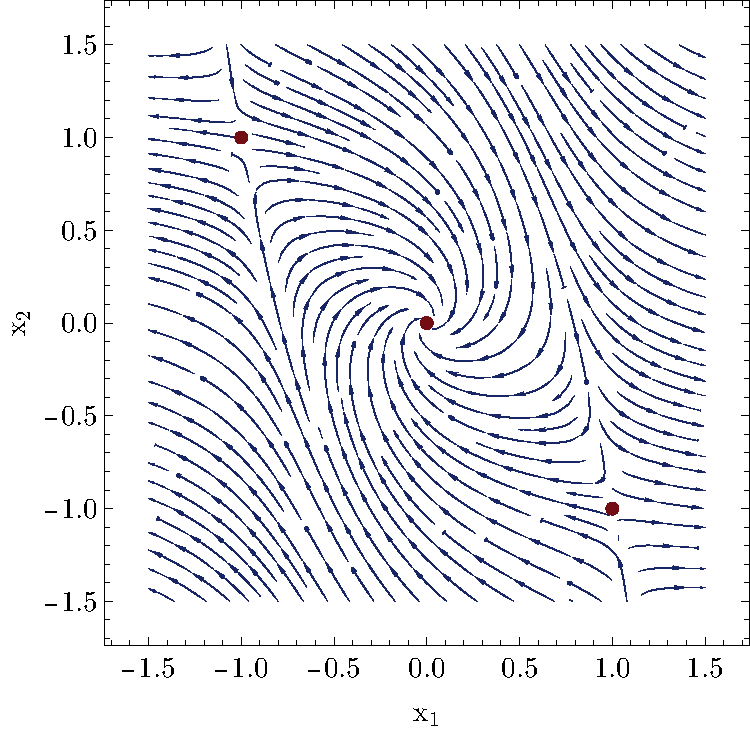
\includegraphics[width=\figwidth]{../images/p1.pdf}
	\caption{Фазовый портрет}
\end{figure}



\subsection{Система 2}

Рассмотрим систему:

\begin{equation} \label{sys:task1_2}
	\begin{cases}
		\dot{x}_1 = x_1 + x_1 x_2 \\
		\dot{x}_2 = -x_2 + x_2^2 + x_1 x_2 - x_1^3
	\end{cases}
\end{equation}

Найдем точки равновесия системы. Положим \(\dot{x}_1 = 0 \text{ и } \dot{x}_2 = 0\):

\[
\begin{cases}
	x_1(1 + x_2) = 0 \\
	-x_2 + x_2^2 + x_1 x_2 - x_1^3 = 0
\end{cases} 
\qquad \Longrightarrow \qquad
\begin{cases}
	x_1 = 0 \text{ или } x_2 = -1 \\
	-x_2 + x_2^2 + x_1 x_2 - x_1^3 = 0
\end{cases}
\]

При \(x_1 = 0\) получаем \(x_2(x_2 - 1) = 0\), откуда \(x_2 = 0\) или \(x_2 = 1\). При \(x_2 = -1\) получаем \(x_1^3 + x_1 - 2 = 0\), единственный действительный корень \(x_1 = 1\). Полученные точки равновесия:

\[
P_1 = (0, 0) \qquad P_2 = (0, 1) \qquad P_3 = (1, -1) 
\]

На основе метода линеаризации в точке определим тип каждого изолированного состояния равновесия. Построим матрицу Якоби:

\[
J(x_1, x_2) = \frac{\partial f}{\partial x} = 
\begin{bmatrix}
	\dfrac{\partial \dot{x}_1}{\partial x_1} & \dfrac{\partial \dot{x}_1}{\partial x_2} \\[10pt]
	\dfrac{\partial \dot{x}_2}{\partial x_1} & \dfrac{\partial \dot{x}_2}{\partial x_2}
\end{bmatrix} = 
\begin{bmatrix}
	1 + x_2 & x_1 \\
	-3x_1^2 + x_2 & x_1 + 2x_2 - 1
\end{bmatrix}
\]

Вычислим матрицу Якоби и её собственные числа $\lambda$ в каждой из найденных точек равновесия.

\begin{itemize}
	\item \(P_1 = (0, 0)\)
	
	\[
	A_1 = J|_{(0,0)} = \begin{bmatrix} 1 & 0 \\ 0 & -1 \end{bmatrix}
	\qquad \Longrightarrow \qquad
	\lambda_{1,2} = 1, -1
	\]
	
	Так как $\lambda_1 > 0$ и $\lambda_2 < 0$, точка $P_1$ --- седло.
	
	\item \(P_2 = (0, 1)\)
	
	\[
	A_2 = J|_{(0,1)} = \begin{bmatrix} 2 & 0 \\ 1 & 1 \end{bmatrix}
	\qquad \Longrightarrow \qquad
	\lambda_{1,2} = 2, 1
	\]
	
	Так как $\lambda_{1,2} > 0$, точка $P_2$ --- неустойчивый узел.
	
	\item \(P_3 = (1, -1)\)
	
	\[
	A_3 = J|_{(1,-1)} = \begin{bmatrix} 0 & 1 \\ -4 & -2 \end{bmatrix}
	\]
	
	Найдем собственные числа:
	\[
	\det(A_3 - \lambda I) = \lambda(\lambda + 2) + 4 = \lambda^2 + 2\lambda + 4 = 0
	\qquad \Longrightarrow \qquad
	\lambda_{1,2} = -1 \pm j\sqrt{3}
	\]
	
	Так как $\text{Re}(\lambda) < 0$, точка $P_3$ --- устойчивый фокус.
	
\end{itemize}

Построим фазовый портрет системы \eqref{sys:task1_2}:

\begin{figure}[H]
	\centering
	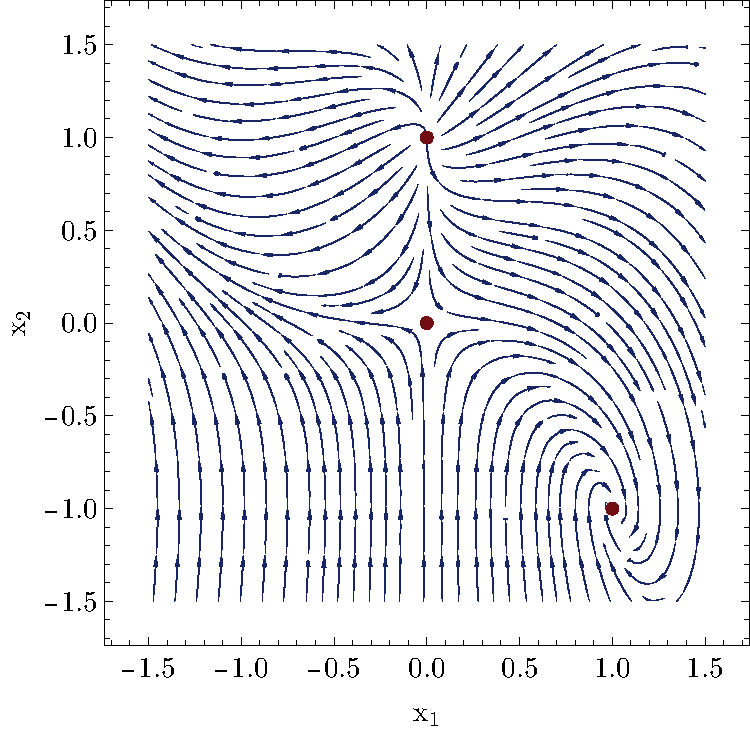
\includegraphics[width=\figwidth]{../images/p2.pdf}
	\caption{Фазовый портрет}
\end{figure}

\subsection{Система 3}

Рассмотрим систему:

\begin{equation} \label{sys:task1_3}
	\begin{cases}
		\dot{x}_1 = x_2 \\
		\dot{x}_2 = -x_1 + x_2(1 - x_1^2 + 0.1x_1^4)
	\end{cases}
\end{equation}

Найдем точки равновесия системы. Положим \(\dot{x}_1 = 0 \text{ и } \dot{x}_2 = 0\):

\[
\begin{cases}
	x_2 = 0 \\
	-x_1 + x_2(1 - x_1^2 + 0.1x_1^4) = 0
\end{cases} 
\qquad \Longrightarrow \qquad
\begin{cases}
	x_2 = 0 \\
	-x_1 = 0
\end{cases}
\]

Полученная точка равновесия:

\[
P_1 = (0, 0)
\]

На основе метода линеаризации в точке определим тип изолированного состояния равновесия. Построим матрицу Якоби:

\[
J(x_1, x_2) = \frac{\partial f}{\partial x} = 
\begin{bmatrix}
	\dfrac{\partial \dot{x}_1}{\partial x_1} & \dfrac{\partial \dot{x}_1}{\partial x_2} \\[10pt]
	\dfrac{\partial \dot{x}_2}{\partial x_1} & \dfrac{\partial \dot{x}_2}{\partial x_2}
\end{bmatrix} = 
\begin{bmatrix}
	0 & 1 \\
	-x_2(2x_1 - 0.4x_1^3) - 1 & 1 - x_1^2 + 0.1x_1^4
\end{bmatrix}
\]

Вычислим матрицу Якоби и её собственные числа $\lambda$ в найденной точке равновесия.

\begin{itemize}
	\item \(P_1 = (0, 0)\)
	
	\[
	A_1 = J|_{(0,0)} = \begin{bmatrix} 0 & 1 \\ -1 & 1 \end{bmatrix}
	\]
	
	Найдем собственные числа:
	\[
	\det(A_1 - \lambda I) = -\lambda(1 - \lambda) + 1 = \lambda^2 - \lambda + 1 = 0
	\qquad \Longrightarrow \qquad
	\lambda_{1,2} = 0.5 \pm j\frac{\sqrt{3}}{2}
	\]
	
	Так как $\text{Re}(\lambda) > 0$, точка $P_1$ --- неустойчивый фокус.
	
\end{itemize}

Построим фазовый портрет системы \eqref{sys:task1_3}:

\begin{figure}[H]
	\centering
	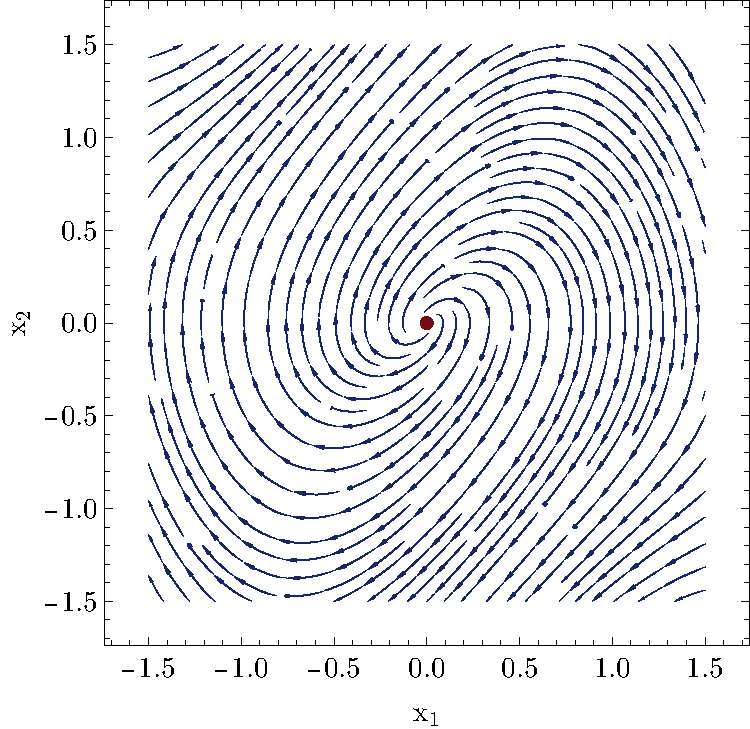
\includegraphics[width=\figwidth]{../images/p3.pdf}
	\caption{Фазовый портрет}
\end{figure}


\subsection{Система 4}

Рассмотрим систему:

\begin{equation} \label{sys:task1_4}
	\begin{cases}
		\dot{x}_1 = (x_1 - x_2)(1 - x_1^2 - x_2^2) \\
		\dot{x}_2 = (x_1 + x_2)(1 - x_1^2 - x_2^2)
	\end{cases}
\end{equation}

Найдем точки равновесия системы. Положим \(\dot{x}_1 = 0 \text{ и } \dot{x}_2 = 0\). Система обращается в ноль при \(1 - x_1^2 - x_2^2 = 0\) или при \(x_1 = x_2 = 0\). Изолированная точка равновесия:

\[
P_1 = (0, 0)
\]

Построим матрицу Якоби:

\[
J(x_1, x_2) = 
\begin{bmatrix}
	1 - 3x_1^2 - x_2^2 + 2x_1x_2 & -1 + x_1^2 - 2x_1x_2 + 3x_2^2 \\[6pt]
	1 - 3x_1^2 - x_2^2 - 2x_1x_2 & 1 - x_1^2 - 3x_2^2 - 2x_1x_2
\end{bmatrix}
\]

Вычислим собственные числа в точке \(P_1\):

\[
A_1 = J|_{(0,0)} = \begin{bmatrix} 1 & -1 \\ 1 & 1 \end{bmatrix}
\qquad \Longrightarrow \qquad
\lambda_{1,2} = 1 \pm j
\]

Линеаризация предсказывает неустойчивый фокус. Для уточнения устойчивости используем переход к полярным координатам \(x_1 = r \cos \theta\), \(x_2 = r \sin \theta\):

\[
r \dot{r} = x_1 \dot{x}_1 + x_2 \dot{x}_2 = r^2(1 - r^2)
\qquad \Longrightarrow \qquad
\dot{r} = r(1 - r^2)
\]

\[
r^2 \dot{\theta} = x_1 \dot{x}_2 - x_2 \dot{x}_1 = r^2(1 - r^2)
\qquad \Longrightarrow \qquad
\dot{\theta} = 1 - r^2
\]

При \(0 < r < 1\) имеем \(\dot{r} > 0\), траектории удаляются от начала координат. При \(r = 1\) имеем \(\dot{r} = 0\), что соответствует окружности состояний равновесия. Точка \(P_1(0,0)\) является неустойчивым фокусом.

Построим фазовый портрет системы \eqref{sys:task1_4}:

\begin{figure}[H]
	\centering
	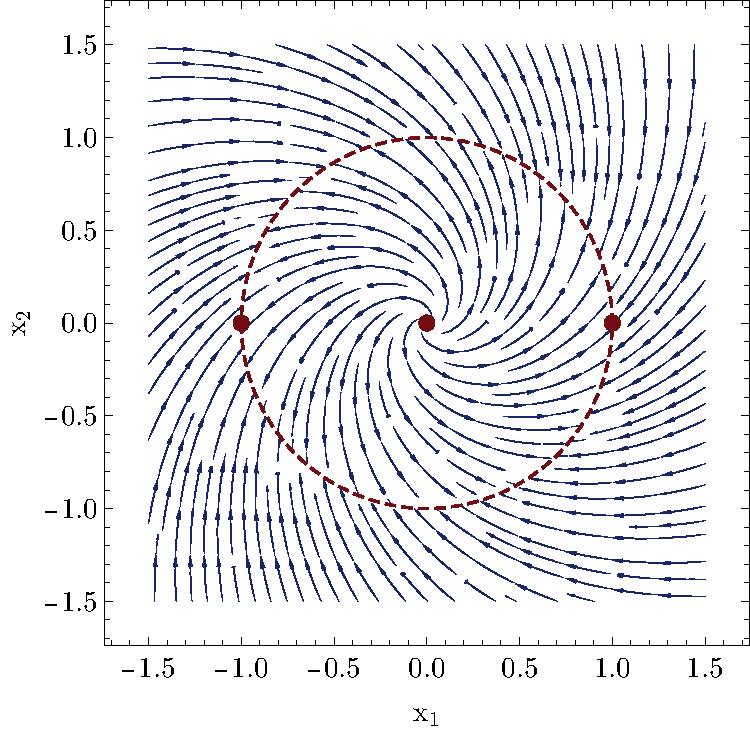
\includegraphics[width=\figwidth]{../images/p4.pdf}
	\caption{Фазовый портрет}
\end{figure}

\subsection{Система 5}

Рассмотрим систему:

\begin{equation} \label{sys:task1_5}
	\begin{cases}
		\dot{x}_1 = -x_1^3 + x_2 \\
		\dot{x}_2 = x_1 - x_2^3
	\end{cases}
\end{equation}

Найдем точки равновесия системы. Положим \(\dot{x}_1 = 0 \text{ и } \dot{x}_2 = 0\):

\[
\begin{cases}
	x_2 = x_1^3 \\
	x_1 = x_2^3
\end{cases} 
\qquad \Longrightarrow \qquad
x_1 = x_1^9
\qquad \Longrightarrow \qquad
x_1(x_1^8 - 1) = 0
\]

Действительные корни: \(x_1 = 0, 1, -1\). Полученные точки равновесия:

\[
P_1 = (0, 0) \qquad P_2 = (1, 1) \qquad P_3 = (-1, -1) 
\]

На основе метода линеаризации в точке определим тип каждого изолированного состояния равновесия. Построим матрицу Якоби:

\[
J(x_1, x_2) = \frac{\partial f}{\partial x} = 
\begin{bmatrix}
	\dfrac{\partial \dot{x}_1}{\partial x_1} & \dfrac{\partial \dot{x}_1}{\partial x_2} \\[10pt]
	\dfrac{\partial \dot{x}_2}{\partial x_1} & \dfrac{\partial \dot{x}_2}{\partial x_2}
\end{bmatrix} = 
\begin{bmatrix}
	-3x_1^2 & 1 \\
	1 & -3x_2^2
\end{bmatrix}
\]

Вычислим матрицу Якоби и её собственные числа $\lambda$ в каждой из найденных точек равновесия.

\begin{itemize}
	\item \(P_1 = (0, 0)\)
	
	\[
	A_1 = J|_{(0,0)} = \begin{bmatrix} 0 & 1 \\ 1 & 0 \end{bmatrix}
	\qquad \Longrightarrow \qquad
	\lambda_{1,2} = 1, -1
	\]
	
	Так как $\lambda_1 > 0$ и $\lambda_2 < 0$, точка $P_1$ --- седло.
	
	\item \(P_2 = (1, 1)\)
	
	\[
	A_2 = J|_{(1,1)} = \begin{bmatrix} -3 & 1 \\ 1 & -3 \end{bmatrix}
	\]
	
	Найдем собственные числа:
	\[
	\det(A_2 - \lambda I) = (-3-\lambda)^2 - 1 = \lambda^2 + 6\lambda + 8 = 0
	\qquad \Longrightarrow \qquad
	\lambda_{1,2} = -2, -4
	\]
	
	Так как $\lambda_{1,2} < 0$, точка $P_2$ --- устойчивый узел.
	
	\item \(P_3 = (-1, -1)\)
	
	\[
	A_3 = J|_{(-1,-1)} = \begin{bmatrix} -3 & 1 \\ 1 & -3 \end{bmatrix}
	\qquad \Longrightarrow \qquad
	\lambda_{1,2} = -2, -4
	\]
	
	Так как $\lambda_{1,2} < 0$, точка $P_3$ --- устойчивый узел.
	
\end{itemize}

Построим фазовый портрет системы \eqref{sys:task1_5}:

\begin{figure}[H]
	\centering
	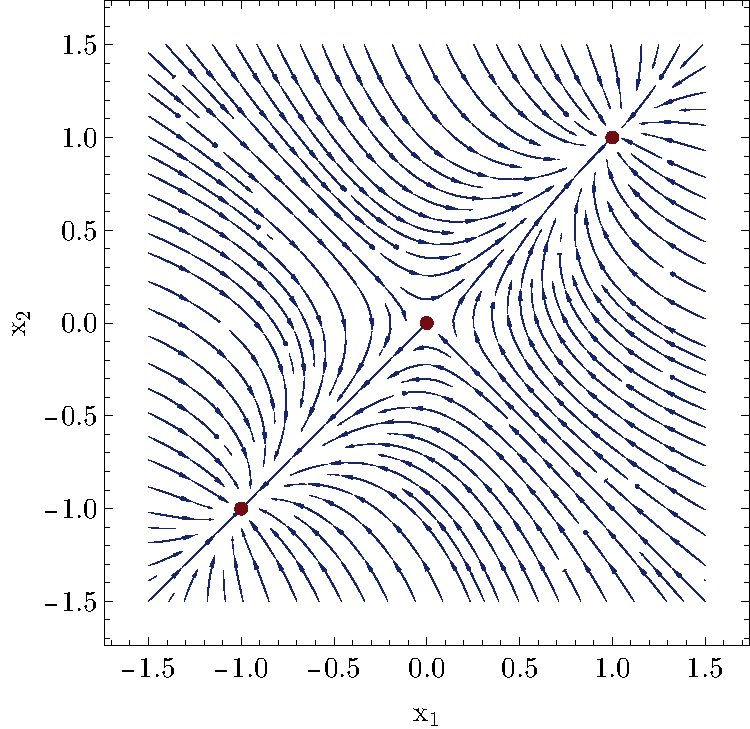
\includegraphics[width=\figwidth]{../images/p5.pdf}
	\caption{Фазовый портрет}
\end{figure}


\subsection{Система 6}

Рассмотрим систему:

\begin{equation} \label{sys:task1_6}
	\begin{cases}
		\dot{x}_1 = -x_1^3 + x_2^3 \\
		\dot{x}_2 = x_2^3 x_1 - x_2^3
	\end{cases}
\end{equation}

Найдем точки равновесия системы. Положим \(\dot{x}_1 = 0 \text{ и } \dot{x}_2 = 0\):

\[
\begin{cases}
	x_2^3 = x_1^3 \\
	x_2^3(x_1 - 1) = 0
\end{cases} 
\qquad \Longrightarrow \qquad
\begin{cases}
	x_2 = x_1 \\
	x_1^3(x_1 - 1) = 0
\end{cases}
\]

Действительные корни: \(x_1 = 0, 1\). Полученные точки равновесия:

\[
P_1 = (0, 0) \qquad P_2 = (1, 1)
\]

На основе метода линеаризации в точке определим тип каждого изолированного состояния равновесия. Построим матрицу Якоби:

\[
J(x_1, x_2) = \frac{\partial f}{\partial x} = 
\begin{bmatrix}
	\dfrac{\partial \dot{x}_1}{\partial x_1} & \dfrac{\partial \dot{x}_1}{\partial x_2} \\[10pt]
	\dfrac{\partial \dot{x}_2}{\partial x_1} & \dfrac{\partial \dot{x}_2}{\partial x_2}
\end{bmatrix} = 
\begin{bmatrix}
	-3x_1^2 & 3x_2^2 \\
	x_2^3 & 3x_1 x_2^2 - 3x_2^2
\end{bmatrix}
\]

Вычислим матрицу Якоби и её собственные числа $\lambda$ в каждой из найденных точек равновесия.

\begin{itemize}
	\item \(P_1 = (0, 0)\)
	
	\[
	A_1 = J|_{(0,0)} = \begin{bmatrix} 0 & 0 \\ 0 & 0 \end{bmatrix}
	\qquad \Longrightarrow \qquad
	\lambda_{1,2} = 0, 0
	\]
	
	Так как собственные числа нулевые, метод линеаризации не дает ответа об устойчивости.
	
	\item \(P_2 = (1, 1)\)
	
	\[
	A_2 = J|_{(1,1)} = \begin{bmatrix} -3 & 3 \\ 1 & 0 \end{bmatrix}
	\]
	
	Найдем собственные числа:
	\[
	\det(A_2 - \lambda I) = -\lambda(-3-\lambda) - 3 = \lambda^2 + 3\lambda - 3 = 0
	\qquad \Longrightarrow \qquad
	\lambda_{1,2} = \frac{-3 \pm \sqrt{21}}{2} \approx 0.79, -3.79
	\]
	
	Так как $\lambda_1 > 0$ и $\lambda_2 < 0$, точка $P_2$ --- седло.
	
\end{itemize}

Построим фазовый портрет системы \eqref{sys:task1_6}:

\begin{figure}[H]
	\centering
	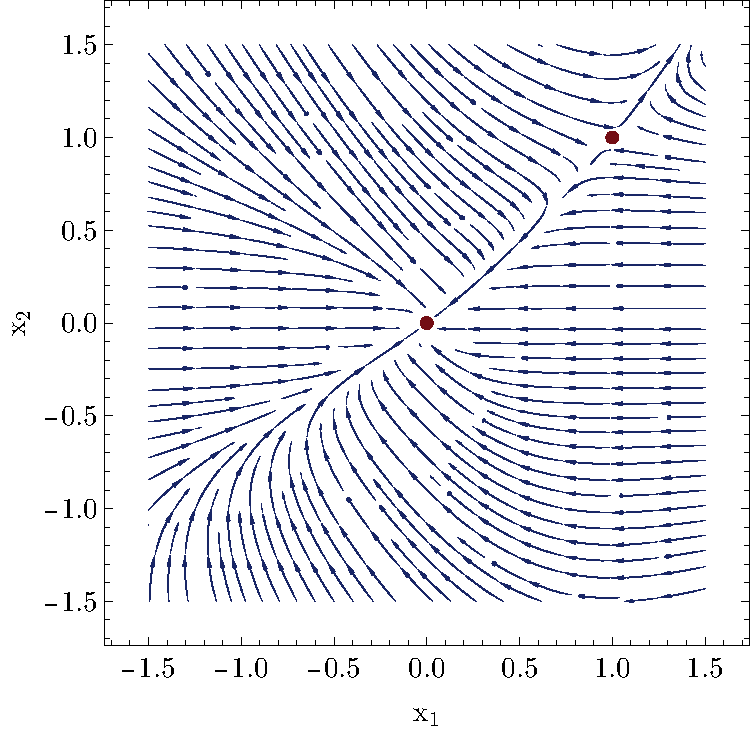
\includegraphics[width=\figwidth]{../images/p6.pdf}
	\caption{Фазовый портрет}
\end{figure}


\subsection{Система 7}

Рассмотрим систему:

\[
\begin{cases}
	\dot{x}_1 = -x_1^3 + x_2^3 \\
	\dot{x}_2 = x_1 + 3x_3 - x_2^3 \\
	\dot{x}_3 = x_1 x_3 - x_2^3 - \sin(x_1)
\end{cases}
\]

Найдем точки равновесия системы. Положим \(\dot{x}_1 = 0\), \(\dot{x}_2 = 0\) и \(\dot{x}_3 = 0\):

\[
\begin{cases}
	x_2^3 = x_1^3 \\
	x_1 + 3x_3 - x_2^3 = 0 \\
	x_1 x_3 - x_2^3 - \sin(x_1) = 0
\end{cases}
\qquad \Longrightarrow \qquad
\begin{cases}
	x_2 = x_1 \\
	x_3 = \dfrac{x_1^3 - x_1}{3} \\[8pt]
	\dfrac{x_1^4 - x_1^2}{3} - x_1^3 - \sin(x_1) = 0
\end{cases}
\]

Функция \(g(x_1) = \dfrac{x_1^4}{3} - x_1^3 - \dfrac{x_1^2}{3} - \sin(x_1)\) имеет единственный действительный корень \(x_1 = 0\). Единственная точка равновесия:

\[
P_1 = (0, 0, 0)
\]

Построим матрицу Якоби:

\[
J(x_1, x_2, x_3) = 
\begin{bmatrix}
	-3x_1^2 & 3x_2^2 & 0 \\
	1 & -3x_2^2 & 3 \\
	x_3 - \cos(x_1) & -3x_2^2 & x_1
\end{bmatrix}
\]

Вычислим собственные числа в точке \(P_1\):

\[
A_1 = J|_{(0,0,0)} = \begin{bmatrix} 0 & 0 & 0 \\ 1 & 0 & 3 \\ -1 & 0 & 0 \end{bmatrix}
\qquad \Longrightarrow \qquad
\lambda_{1,2,3} = 0, 0, 0
\]

Так как все собственные числа равны нулю, метод линеаризации не дает ответа об устойчивости. 


\newpage
\section{Синтез локально стабилизирующего регулятора}


Рассмотрим систему \eqref{sys:task1_1} с управлением:
\[
\begin{cases}
	\dot{x}_1 = -x_1 + 2x_1^3 + x_2 + \sin u_1 \\
	\dot{x}_2 = -x_1 - x_2 + 3\sin u_2
\end{cases}
\]

Выберем для стабилизации седловую точку равновесия $P_2(1, -1)$. Линеаризация нелинейной системы в окрестности состояния $x^* = (1, -1)$ и управления $u^* = (0, 0)$ выполняется путем вычисления матриц Якоби по состоянию и управлению:

\[
\begin{aligned}
	A &= \left. \frac{\partial f}{\partial x} \right|_{x^*, u^*} = \begin{bmatrix} 5 & 1 \\ -1 & -1 \end{bmatrix} \\[10pt]
	B &= \left. \frac{\partial f}{\partial u} \right|_{x^*, u^*} = \begin{bmatrix} 1 & 0 \\ 0 & 3 \end{bmatrix}
\end{aligned}
\]

Проверим управляемость системы. Матрица управляемости:

\[
\mathcal{C} = \begin{bmatrix} B & AB \end{bmatrix} = 
\begin{bmatrix}
	1 & 0 & 5 & 3 \\
	0 & 3 & -1 & -3
\end{bmatrix}
\]

Так как $\text{rank}(\mathcal{C}) = 2$, что равно размерности системы, исходная система является полностью управляемой. Значит мы можем синтезировать стабилизирующий регулятор.\\

Зададимся желаемым спектром системы:

\[
\sigma(A-BK) = \{-5,-6\}
\]
Методом размещения полюсов \texttt{place()} находим матрицу обратной связи:
\[
K = \begin{bmatrix} 10 & 1 \\[4pt]
	-\dfrac{1}{3} & \dfrac{5}{3} \end{bmatrix}
\]

Закон управления строится относительно отклонений $\tilde{x} = x - x^*$ с ограничением $|u_i| \le 3$ для предотвращения насыщения нелинейных звеньев. Результаты моделирования нелинейной замкнутой системы при $x(0) = \begin{bmatrix}
	1.1 \\
	-0.9
\end{bmatrix}$ представлены на рисунках ниже.

\begin{figure}[H]
	\centering
	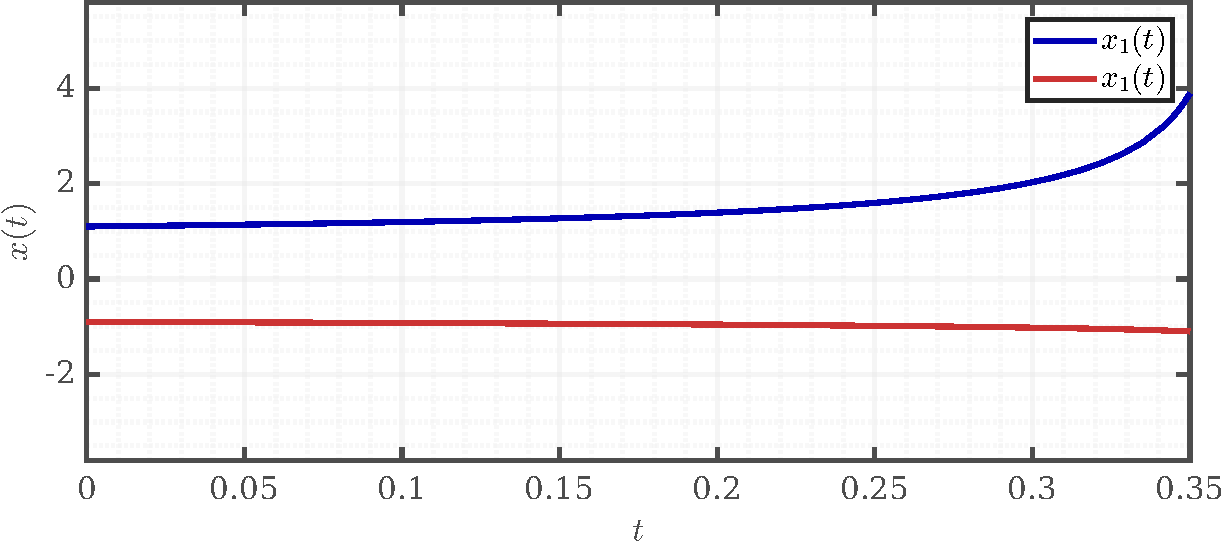
\includegraphics[width=0.7\textwidth]{../images/xop1.pdf}
	\caption{Разомкнутая система}
\end{figure}

\begin{figure}[H]
	\centering
	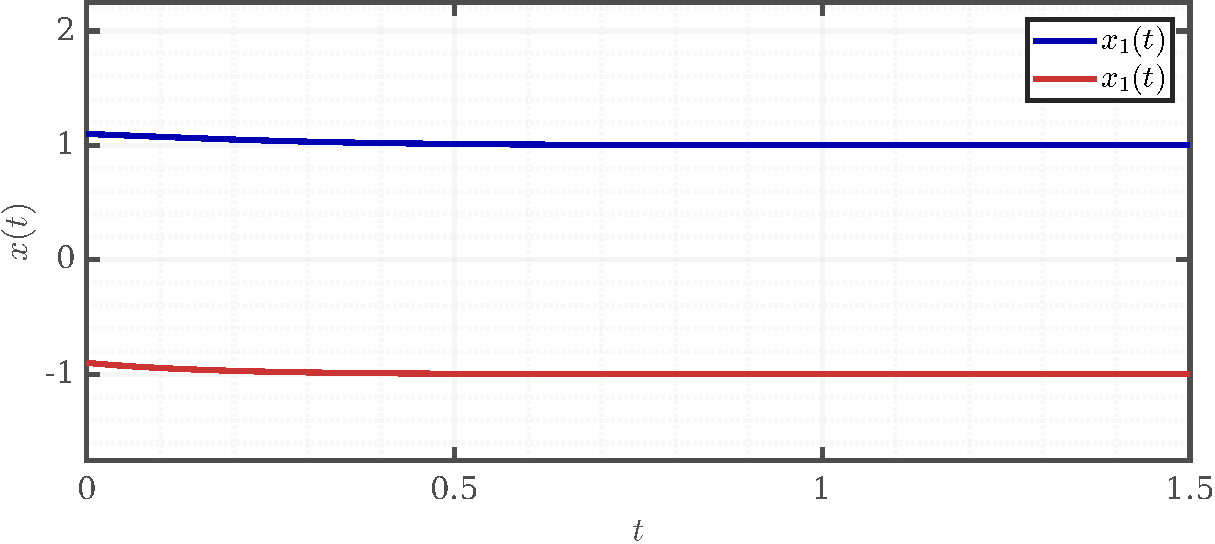
\includegraphics[width=0.7\textwidth]{../images/xcl1.pdf}
	\caption{Замкнутая система}
\end{figure}



\newpage
\section{Вывод}

В первой части работы для семи нелинейных систем найдены все изолированные точки равновесия, построены матрицы Якоби и вычислены собственные числа. На их основе определены типы состояний равновесия. Для случаев с нулевыми или чисто мнимыми собственными числами показано, что линеаризация не дает полного ответа об устойчивости.

Во второй части для первой системы синтезирован локально стабилизирующий регулятор в ненулевой точке равновесия $(1, -1)$. Проверена управляемость линеаризованной модели, рассчитана матрица обратной связи методом размещения полюсов. Численное моделирование подтвердило работоспособность регулятора и асимптотическую сходимость траекторий к заданному состоянию.










\newpage
\section{Приложение}

\subsection*{Задание 1}


\begin{lstlisting}[
	style = Matlab-editor, 
	caption={Алгоритм численного поиска точек равновесия и определения их типа через собственные числа матрицы Якоби}, 
	label={lst:jacobian_analysis}
	]	
clc; clear;
syms x1 x2 real

systems = {
	{[-x1 + 2*x1^3 + x2; -x1 - x2], [x1; x2]};
	{[x1 + x1*x2; -x2 + x2^2 + x1*x2 - x1^3], [x1; x2]};
	{[x2; -x1 + x2*(1-x1^2+0.1*x1^4)], [x1; x2]};
	{[(x1-x2)*(1-x1^2-x2^2); (x1+x2)*(1-x1^2-x2^2)], [x1; x2]};
	{[-x1^3 + x2; x1 - x2^3], [x1; x2]};
	{[-x1^3 + x2^3; x2^3*x1 - x2^3], [x1; x2]}
};

for i = 1:length(systems)
	fprintf("> System %0d", i); fprintf("\n");
	sys  = systems{i}{1};
	vars = systems{i}{2}; 
	
	sol = solve(sys == 0, vars, 'Real', true);
	
	pts = [];
	for v = 1:length(vars)
		pts = [pts, double(sol.(char(vars(v))))];
	end;
	pts
	
	J = jacobian(sys, vars)
	fprintf("\n");
	
	for k = 1:size(pts, 1)
		fprintf(">> point %0d", k); fprintf("\n");
		Ak = subs(J, vars.', pts(k, :)) 
		fprintf("\n");
		eig_vals = eig(double(Ak))
		fprintf("\n");
	end;

end;
\end{lstlisting}





\end{document}